\section{数据处理与统一物理规则}

\noindent\textbf{人工智能辅助说明：}本节及后文的附件数据分析、计算程序和初稿曾使用 OpenAI Codex 辅助（GPT-5，开发机构 OpenAI；该模型于 2025 年 8 月 7 日发布）。参赛队已对采用的建模思路、公式、代码和文字进行理解、复核与改写；下述数值均由随附程序重新计算并回代检查。

\subsection{数据核对与空间计算}

附件的逐箱清单共80行，逐箱编号均不重复，总载质量758~kg，总体积2.011~m$^3$。调度中心记为O01，服务区记为S001至S015。实体运输机为A型4架、B型2架、C型2架；共享电池库存为6、4、4组。另有R型中继机2架和共享能源组件6组。DEM是EPSG:4326坐标系的1309$\times$1486个30米名义分辨率像元，其地理范围覆盖全部任务节点；Copernicus DEM产品资料作为题目所列高程数据来源背景，栅格尺寸和坐标信息以实际附件为准\cite{copernicus}。坐标以WGS84椭球计算测地距离，路线规划不使用道路数据。

DEM地形、调度中心、服务区以及道路和水系等地理要素的相对位置见图~\ref{fig:node_map}。该图用于呈现任务空间与地形背景，实际航段能耗仍由后文给出的栅格穿越和逐段计算确定。
\begin{figure}[H]\centering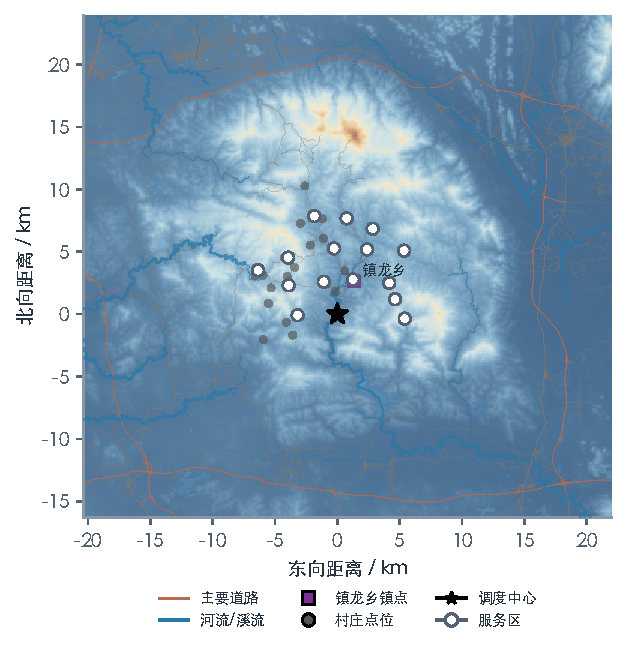
\includegraphics[width=.92\textwidth]{../figures/paper_full_20260926/q1_dem_nodes.pdf}\caption{DEM地形、地理要素与任务服务点分布}\label{fig:node_map}\end{figure}

\begin{table}[H]\centering\normalsize
\caption{原始附件的用途及进入模型的位置}\label{tab:data_files}
\begin{tabular}{ll}\toprule
数据文件 & 用途\\\midrule
调度中心与服务区.xlsx & 节点坐标、高程及需求区定位\\
物资需求与配送时限.xlsx & 80箱质量、体积、目的地、时限和优先系数\\
运输无人机数据.xlsx & A/B/C机型能力、能量和充电参数\\
中继无人机数据.xlsx & R型机、能源组件、飞行和悬停参数\\
通信链路参数.xlsx & 双向链路预算及遮挡附加损耗\\
30米DEM地形栅格 & 航段最高地形、净空与视线遮挡\\\bottomrule
\end{tabular}\end{table}

80个货箱在各服务区的类别构成不同。医疗或首批保障箱带有硬截止要求，分布见图~\ref{fig:box_deadline_mix}。
\begin{figure}[H]\centering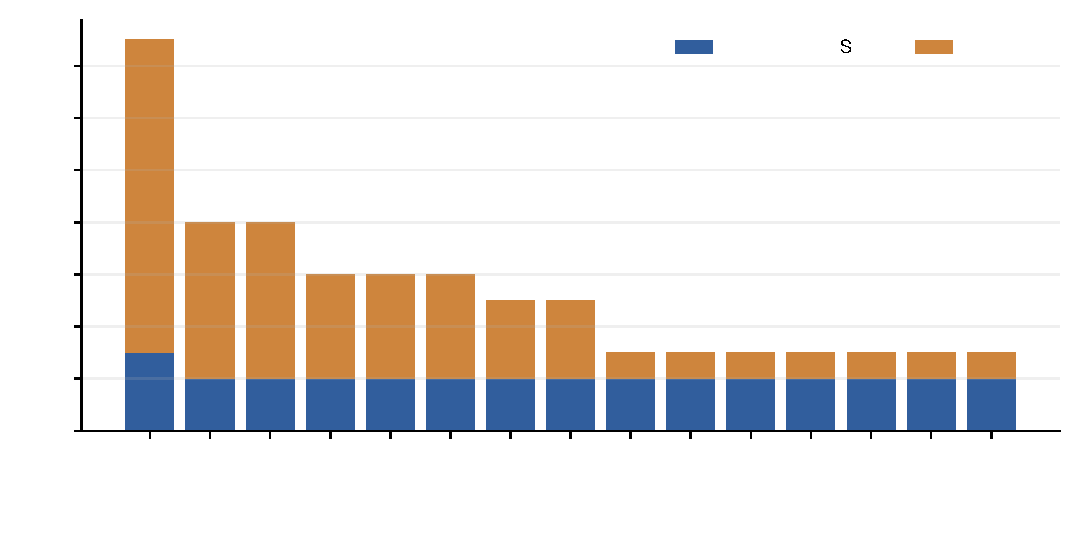
\includegraphics[width=.88\textwidth]{../figures/rigor_pool_20260926/raw_q2_box_deadline_mix.pdf}\caption{各服务区货箱类别与硬截止构成}\label{fig:box_deadline_mix}\end{figure}

\begin{table}[H]\centering\normalsize
\caption{三类运输机的核心输入参数与题给库存}\label{tab:aircraft_parameters}
\begin{tabular}{lrrrrrr}\toprule
机型 & 机体/架 & 电池/组 & 载重/kg & 容积/m$^3$ & 巡航/(m/s) & 单组可用电量/kWh\\\midrule
A & 4 & 6 & 25 & 0.060 & 12 & 4.5\\
B & 2 & 4 & 30 & 0.073 & 15 & 4.0\\
C & 2 & 4 & 80 & 0.250 & 15 & 8.0\\\bottomrule
\end{tabular}\end{table}

公开的专业无人机规格和无线电抗干扰产品资料可用于理解工程应用背景；例如Matrice 350 RTK规格页给出飞行性能指标，Doodle Labs介绍了面向无人系统的干扰规避功能。本文的A/B/C机型能力、通信频率和链路门限仍完全采用题目附件，未以这些产品数据替代\cite{djiM350,doodleSense}。

不同机型与电池的题给库存是问题二实体排程和问题四独立配置的共同上限，图~\ref{fig:initial_inventory}将其按资源类型列出。
\begin{figure}[H]\centering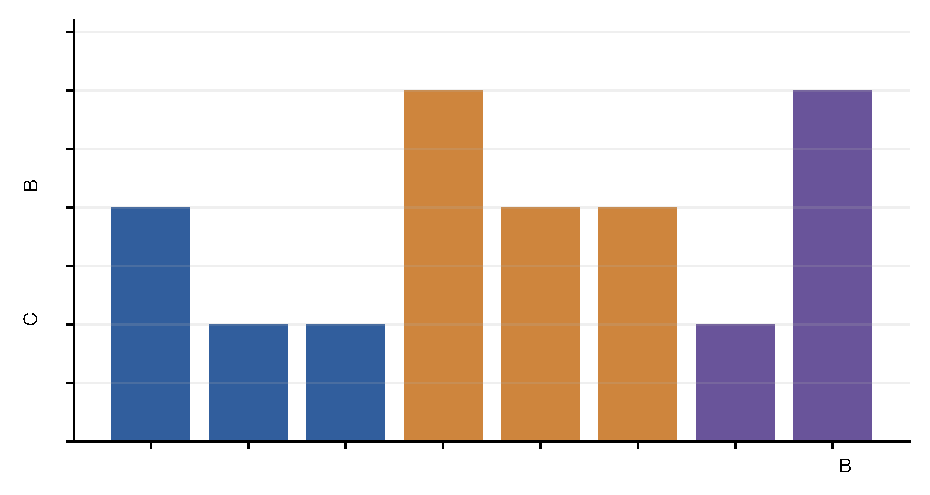
\includegraphics[width=.78\textwidth]{../figures/rigor_pool_20260926/raw_q4_initial_inventory.pdf}\caption{运输机、中继机及共享能源资源的初始库存}\label{fig:initial_inventory}\end{figure}

两节点航段水平投影采用题设直线。我们求出直线与所有经纬网格线的交点，将其分割成位于单个像元内的子段，逐段读取DEM，令巡航海拔为沿线最高地面高程上方50~m。这样不会因稀疏采样跳过窄山脊。调度中心的作业高度为地面高程，服务区的作业高度为地面高程上方30~m。每一次站点交接之后重新由该站作业高度爬升。

\subsection{飞行时间和能耗}

对于机型$g$及起飞后当前有效载荷$q$，采用题给等效航程
\begin{equation}
L_g(q)=L_g^0-(L_g^0-L_g^F)\left(\frac{q}{Q_g}\right)^{3/2}.
\label{eq:range}
\end{equation}
记航段$i\to j$的水平长度为$d_{ij}$，计划巡航海拔为$H_{ij}$，两端作业海拔为$z_i,z_j$，则爬升和下降高度分别为$H_{ij}-z_i$与$H_{ij}-z_j$。题面只写出水平与爬升能耗之和而未展开两项，本文明确采用标准航程标定的单位距离耗电和重力势能折算：
\begin{align}
t^g_{ij}&=\frac{H_{ij}-z_i}{v_g^\uparrow}+\frac{d_{ij}}{v_g^c}+\frac{H_{ij}-z_j}{v_g^\downarrow},\\
E^g_{ij}(q)&=E_g^{\rm use}\frac{d_{ij}}{L_g(q)}+\frac{(m_g+q)9.81(H_{ij}-z_i)}{3.6\times10^6\eta_g}.
\label{eq:energy}
\end{align}
其中$E_g^{\rm use}$是单组电池可用能量，$m_g$为含电池空载质量，$\eta_g$为爬升能耗效率。下降不另计附加能耗。每个架次的航段能量之和须不超过$(1-\rho_g)E_g^{\rm use}$。多点架次在某站交接后立即扣去该站箱重，再计算下一航段。

两篇参考文献为载荷相关能耗提供了物理解释和适用边界。Dorling等由多旋翼悬停诱导功率推得
\begin{equation}
P_{\rm hov}(m)=(W+m)^{3/2}\sqrt{\frac{g^3}{2\rho_a\varsigma n}},\qquad
P_{\rm hov}(m)\approx \alpha m+\beta,
\label{eq:dorling}
\end{equation}
其中$W$为机架质量，$m$为电池与载荷质量，$n$为旋翼数，$\varsigma$为单个旋翼盘面积。对其Hexa-B样机，在$m=0$--$3$~kg范围内拟合得$\alpha=46.7$~W/kg、$\beta=26.9$~W；该文还用飞行测试检验了悬停功率对飞行功率的近似。Zhang等综述的无风稳态平飞升阻比模型则给出单位距离能耗
\begin{equation}
E_{\rm pm}=\frac{(m_{\rm body}+m_{\rm battery}+m_{\rm payload})g}{r\eta}
 +\frac{P_{\rm avio}}{v_a},
\label{eq:epm_literature}
\end{equation}
其中$r$为升阻比，$\eta$为电池至推进系统的能量传递效率，$P_{\rm avio}$为航电功率，$v_a$为空速。该综述比较的不同模型即使在相近条件下也会产生明显不同的能耗估计，并指出爬升、下降、悬停、风和航电会改变整次任务的能量需求\cite{dorling,zhang}。因此，这些公式支持“载荷影响能耗”及按飞行阶段核算的建模方向，但其样机系数、旋翼几何和巡航参数无法直接移植到题目给出的三种机型。本文水平能耗仍按题给各机型的载荷—等效航程曲线计算，爬升另按重力势能折算；参考公式不作为未标定参数的替代来源。

准备与逐箱装载时间计入起飞前占用；站点交接时间是“基础时间+逐箱时间”，本站所有箱的交付时刻统一记为交接结束。这一做法对时间窗保守。题设没有运输机交接悬停功率和准备工位数量，因此没有增设未经给定的能耗或工位容量参数。

\subsection{电池与通信状态}

任何电池或中继能源组件均初始满电。一次任务结束后SOC为$1-E/E^{\rm use}$；再次装机前须按题给两阶段线性充电模型恢复100\%。锂离子电池控制资料展示了恒流、恒压分阶段充电的一种工程实现，可作一般技术背景；本文充电阶段、比例和时长仍以题目参数为准\cite{tiCharger}。使用、充电两个区间均占用该组件，且同类电池不可跨机型调配。运输机和中继机的实际架次时间区间亦不得重叠。

固定网关与运输机、中继机之间的双向链路门限分别为122、126~dB，运输机与中继机之间为116~dB。视线受DEM遮挡时在自由空间损耗上增加10~dB，而非直接判为中断。每一时刻运输机必须满足网关直连，或同时满足接入中继与中继回传两条链路。自由空间损耗使用题给的2400~MHz公式，并以实际三维距离计算\cite{itur}。无人机辅助无线通信也被研究为基础设施覆盖不足时的通信方式；本文则通过题给链路预算和直连/中继约束进行具体判定\cite{zeng}。

三类双向链路的允许损耗门限不同，运输机到中继链路的门限最低。图~\ref{fig:link_budgets}汇总题给链路预算，后续通信判定均按对应链路类型分别核验。
\begin{figure}[H]\centering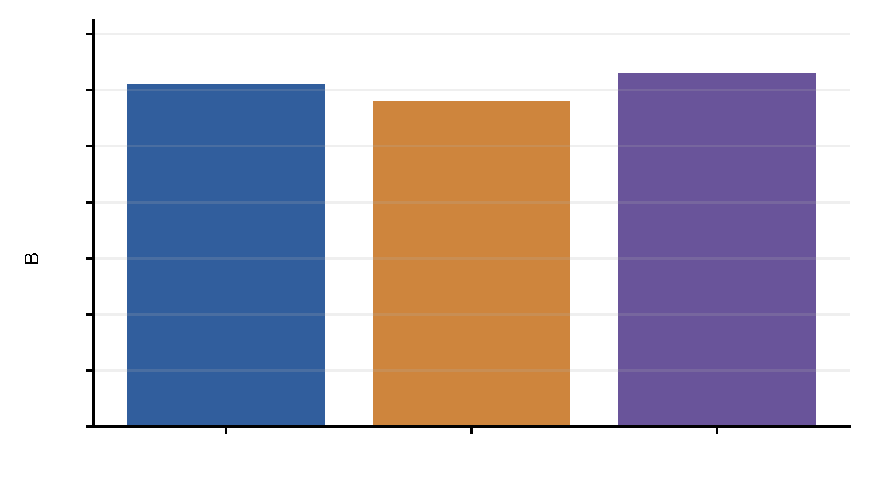
\includegraphics[width=.68\textwidth]{../figures/rigor_pool_20260926/raw_q3_link_budgets.pdf}\caption{运输机与中继通信链路的允许损耗门限}\label{fig:link_budgets}\end{figure}

后续求解严格区分概念模型和实现证据：问题二由路线列启发式生成完整箱组与站序，再由固定路线CP-SAT安排实体资源；问题三以连续区间证书修复通信可行性，并只在归档的有限运输族和中继窗口上协调。因而“可回放可行”与“全空间最优”在表述中始终分开。
